\chapter{Background Estimation}

\label{ch:background}
% --------------------------------------------------------------------------------

The event selection discussed in the previous section focuses on detector signatures, emphasizing a single high-momentum, highly-ionizing track.
That track is then required to be inconsistent with the expected properties of \ac{SM} particles, with various requirements designed to reject jets, hadrons, electrons, and muons (Section~\ref{sec:sm_rejection}).
Therefore the background for this search comes entirely from backgrounds that are outliers of various distributions including $\dedx$, \emfrac, and \ptcone.
The simulation can be tuned in various ways to do an excellent job of modeling the average properties of each particle type~\cite{atlas_sim}, but it is not necessarily expected to accurately reproduce outliers.
For this reasons, the background estimation used for this search is estimated entirely using data.

\section{Background Sources}
\label{sec:background_sources}
\ac{SM} charged particles with lifetimes long enough to form tracks in the inner detector can be grouped into three major categories based on their detector interactions: hadrons, electrons, and muons. 
Every particle that contributes to the background for this search belongs to one of these types.
Relatively pure samples of tracks from each of these types can be formed in data by inverting the various rejection techniques in Section~\ref{sec:sm_rejection}.
Specifically, muons are selected requiring medium muon identification, electrons requiring $\ep > 1.0$ and $\emfrac > 0.95$, and hadrons requiring $\ep > 1.0$ and $\emfrac < 0.95$. 

Figure~\ref{fig:background_species} shows the distributions of momentum and \dedx for these categories in data, after requiring the event level selection as well as the track requirements on $\pt$, hits, and \Nsplit, as discussed in Section~\ref{sec:track_requirements}.
Simulated signal events are included for reference.
These distribution are only illustrative of the differences between types, as the rejection requirements could alter their shape. 
This is especially significant for momentum which enters directly into \ep and can indirectly affect muon identification.
However it is clear that there are some differences between types in both distributions, even though the trends are similar.
The distributions of momentum are not necessarily expected to match between the various types because the production mechanisms for each type result in different kinematic distributions.
\dedx is also different between types because of incomplete isolation; although the requirement on $\Nsplit$ helps to reduce the contribution of nearby particles it does not completely remove the effect of overlaps.
Muons are better isolated because they do not have the additional particle from hadronization present for hadrons and they are significantly less likely do interact with the detector and produce secondary particles compared to hadrons and electrons.
Thus muons have the smallest fraction of \dedx above the threshold of 1.8 \MeVgcm; hadrons and electrons have a larger fraction above this threshold.

\begin{figure}[h]
\centering
\subfloat[]{
  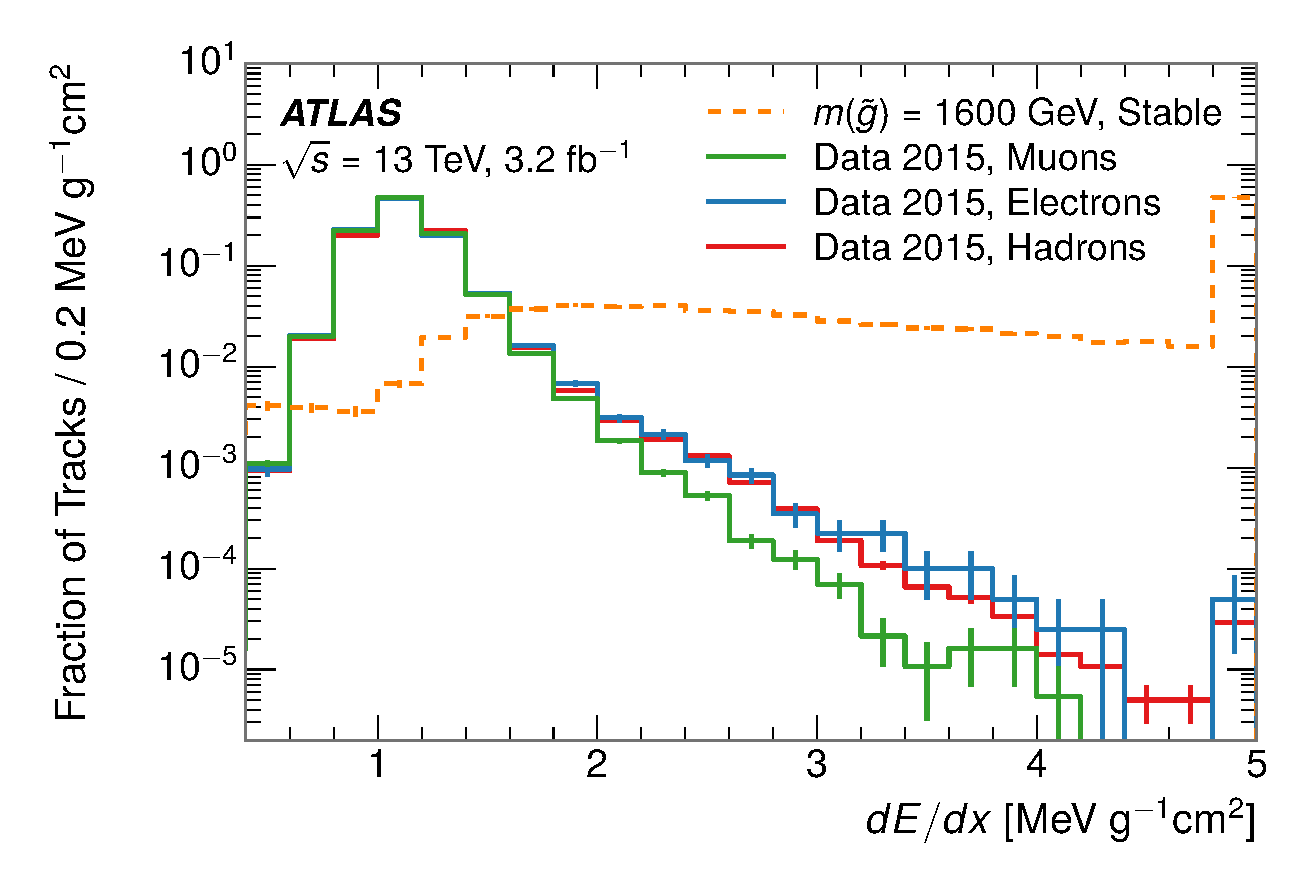
\includegraphics[width=\halffig]{figures/dedx_species.pdf}
}
\subfloat[]{
  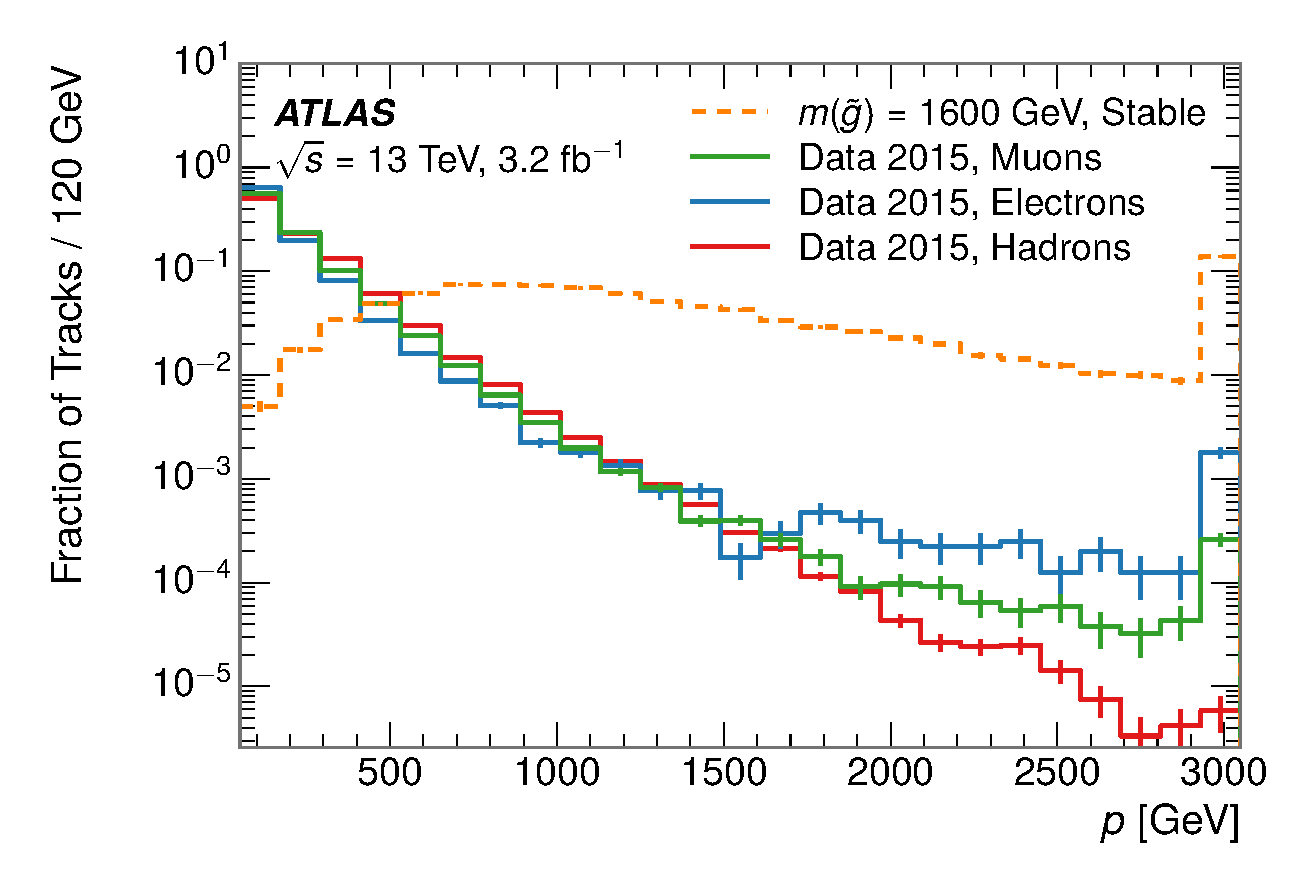
\includegraphics[width=\halffig]{figures/p_species.pdf}
}\\
\caption{The distribution of (a) \dedx and (b) momentum for tracks in data and simulated signal after requiring the event level selection and the track selection on \pt, hits, and \Nsplit. Each sub-figure shows the normalized distributions for tracks classified as hadrons, electrons, and muons in data and \rhadrons in the simulated signal.}
\label{fig:background_species}
\end{figure}

It is difficult to determine what fraction of each particle type enters into the final signal region.
The background method will not have significant dependence on the relative contributions of each species, but it is useful to understand the differences between each when considering the various tests of the method.

% ----------------------------------------

\section{Prediction Method}
\label{sec:background_method}
The data-driven background estimation relies on the independence between the ionization measurement and other kinematic variables in the event.
For standard model particles with momenta above 50 \GeV, \dedx is not correlated with momentum; though there is a slight relativistic rise as momentum increases, the effect is small compared to the width of the distribution of ionization energy deposits..
So, the proposed method to estimate the mass distribution of the signal region is to use the momentum from a track with low \dedx (below the threshold value) and to combine it with a random \dedx value from a \dedx template.
The resulting track is just as likely as the original, so a large set of random generations provide the expected distributions of momentum and ionization.
These are then combined using the parametrization described in Section~\ref{sec:mass_requirement} to estimate $\beta\gamma$ and then form a distribution of mass for the signal region using Equation~\ref{eq:mbetagamma}.

Algorithmically this method is implemented by forming two distinct \acp{CR}.
The first \ac{CR}, CR1, is formed by applying the entire event selection from Chapter~\ref{ch:selection} apart from the \dedx and mass requirements.
The \dedx requirement is instead inverted for this region.
Because of the independence of \dedx and $p$, the tracks in this control region have the same kinematic distribution as the tracks in the signal region, and are used to measure a two-dimensional template of $p$ and $\eta$. 
The second \ac{CR}, CR2, is formed from the event selection through the \dedx requirement, but with an inverted \met requirement.
The tracks in this control region are expected to have similar \dedx distributions as the signal region before the ionization requirement, and so this region is used to measure a two-dimensional template of \dedx and $\eta$. 

The contribution of any signal to the control regions is minimized by the inverted selection requirements.
Only less than 10\% of simulated signal events have either \dedx or \met below the threshold values in the original signal region, while the backgrounds are significantly enhanced by inverting those requirements.
The signal contamination is less than 1\% in both control regions for all of the simulated masses and lifetimes considered in this analysis.

With those measured templates, the shape of the mass estimation is generated by first selecting a random $(p,\ \eta)$ combination from CR1. 
This momentum value is combined with a \dedx value taken from the appropriate distribution of \dedx for the selected $\eta$ from CR2. 
The use of $\eta$ in both random samplings controls for any correlation between $p$, \dedx, and $\eta$. 
Those values are then used to calculate a mass in the same way that is done for regular tracks in data, see Section~\ref{sec:mass_requirement}.
As this procedure includes all \dedx values, the cut at 1.8 \MeVgcm is then enforced to fully model the signal region.
The generated mass distribution is then normalized by scaling the background estimate to the data in the region $M < 160$ \GeV, where signals of this type have already been excluded~\cite{SUSY-2014-09}.
This normalization uses the distributions of mass generated without the ionization requirement.

The statistical uncertainties on these background distributions are calculated by independently fluctuating each bin of the input templates according to their Poisson uncertainties. 
These fluctuations are repeated a large number of times, and the uncertainty on the resulting distribution is taken as the \ac{RMS} deviation of the fluctuations from the average.
As the procedure uses one million random combinations to generate the distributions, The statistical uncertainty from the actual random generations is negligible compared to the uncertainty from measuring the templates.
% ----------------------------------------

\section{Validation}

The validity of the background estimation technique can be evaluated in both data and simulation.
The underlying assumption that random combinations of \dedx and momentum can predict a mass distribution in an orthogonal region can be tested using simulated samples where concerns like multiple particle types can be controlled.
Using the same technique in another set of signal-depleted regions in data then extends this confidence to the more complicated case where several particle species are inherently included.

\subsection{Closure in Simulation}
The first test of the procedure is done using a simulated sample of $W\rightarrow\mu\nu$ decays.
These types of events provide the ingredients required to test the background estimate, \met and isolated tracks, with high statistics.
In this example there is no signal, so simulated events in the orthogonal \acp{CR} are used to estimate the shape of the mass distribution of the simulated events in the signal region.
To reflect the different topology for W boson decays, the \acp{CR} use slightly modified definitions.
In all \acp{CR}, the requirement of $p > 150$ \GeV and the \ac{SM} rejection requirements are removed.
Additionally, for the signal region the requirement on \met is relaxed to 30 \GeV and the corresponding inverted requirement on CR2 is also set at 30 \GeV.

With these modified selections, the simulated and randomly generated distributions of \mdedx are shown in Figure~\ref{fig:closure_mass}. 
This figure includes the mass distributions before and after the requirement on \dedx, which significantly shapes the distributions.
In both cases the background estimation technique reproduces the shape of \mdedx in the signal region.
There is a small difference in the positive tail of the mass distribution prior to the ionization cut, where the random events underestimate the fraction of tracks with mass above 150 \GeV by about 20\%.
After the ionization requirement, however, this discrepancy is not present and the two distributions agree to within statistical uncertainties in the positive tail.

\begin{figure}[h]
\centering
\subfloat[]{
  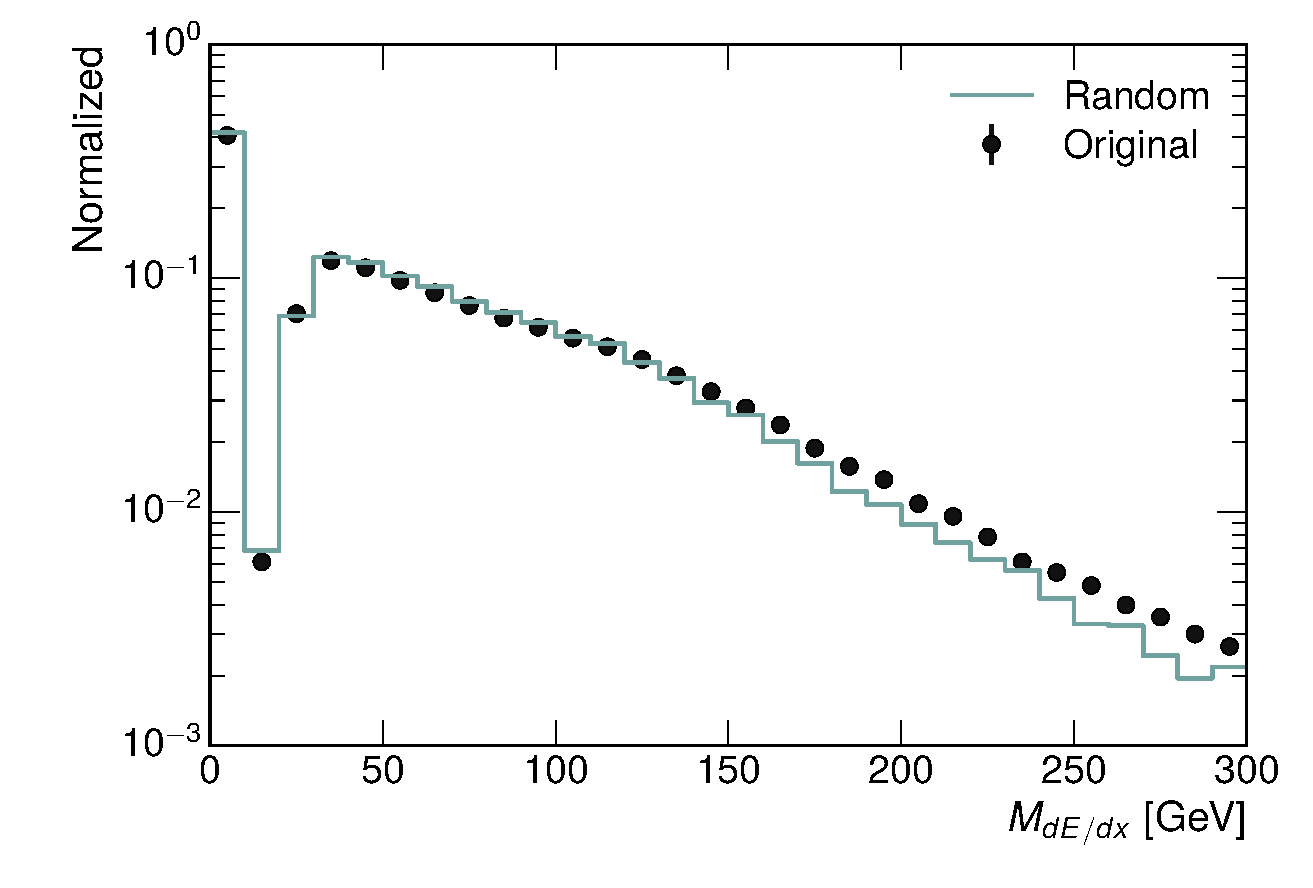
\includegraphics[width=\halffig]{figures/closure_mass_noion.pdf}
}
\subfloat[]{
  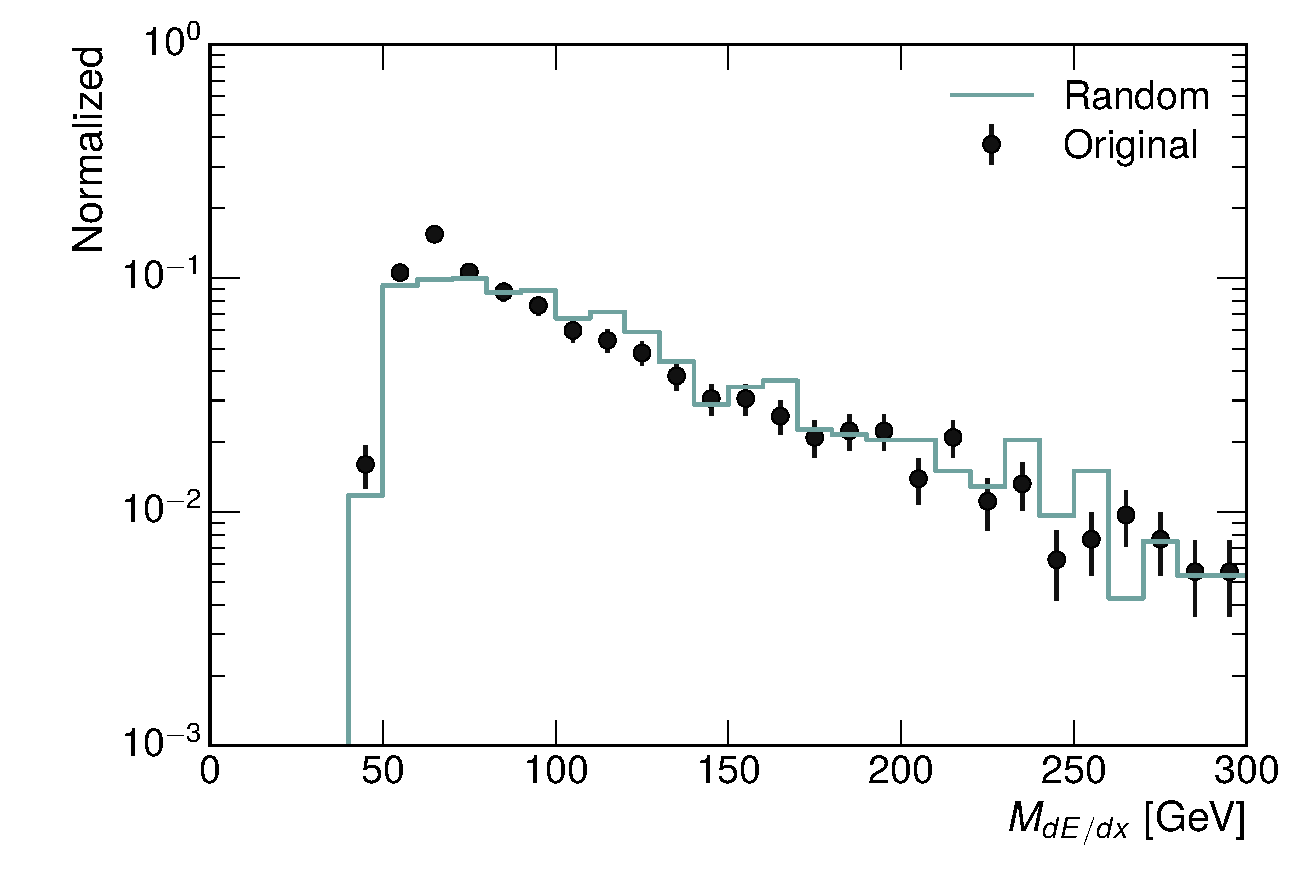
\includegraphics[width=\halffig]{figures/closure_mass.pdf}
}\\
\caption{The distribution of \mdedx (a) before and (b) after the ionization requirement for tracks in simulated W boson decays and for the randomly generated background estimate.}
\label{fig:closure_mass}
\end{figure}

This ability to reproduce the shape of the mass distribution in simulated events shows that the technique works as expected.
No significant biases are acquired in using low \dedx events to select kinematic templates or in using low \met events to select ionization templates, as either would result in a mismodeling of the shape of the mass distribution.
The simulated events contain only one particle type, however, so this test only establishes that the technique works well when the the \acp{CR} are populated by exactly the same species.

\subsection{Validation Region in Data}
The second test of the background estimate is performed using data in an orthogonal validation region.
The validation region, and the corresponding \acp{CR}, are formed using the same selection requirements as in the nominal method but with a modified requirement on momentum, $50 < p [\GeV] < 150$.
This allows the technique to be checked in a region with very similar properties but where the signal is depleted, as the majority of the signal has momentum above 150 \GeV while the backgrounds are enhanced below that threshold.
Any biases on the particle composition of the \acp{CR} for the signal region will be reflected in the \acp{CR} used to estimate the mass distribution in the validation region.

% Show the plots, talk about how the good agreement means the particle species are similar in CR2 

Figure~\ref{fig:validation_mass} shows the measured and randomly generated mass distributions for data before and after the ionization requirement.
The background estimate models the actual background before the ionization requirement very well, with good agreement to within the statistical uncertainties out to the limit of the mass distribution.
There are very few events in the validation region after the ionization requirement, but the few observed events are consistent with the background prediction.
The good agreement in this validation region provides a confirmation that the technique works even in the full-complexity case with multiple particle types entering the distributions.
Any bias from changes in particle composition between regions is small compared to statistical uncertainties.

\begin{figure}[h]
\centering
\subfloat[]{
  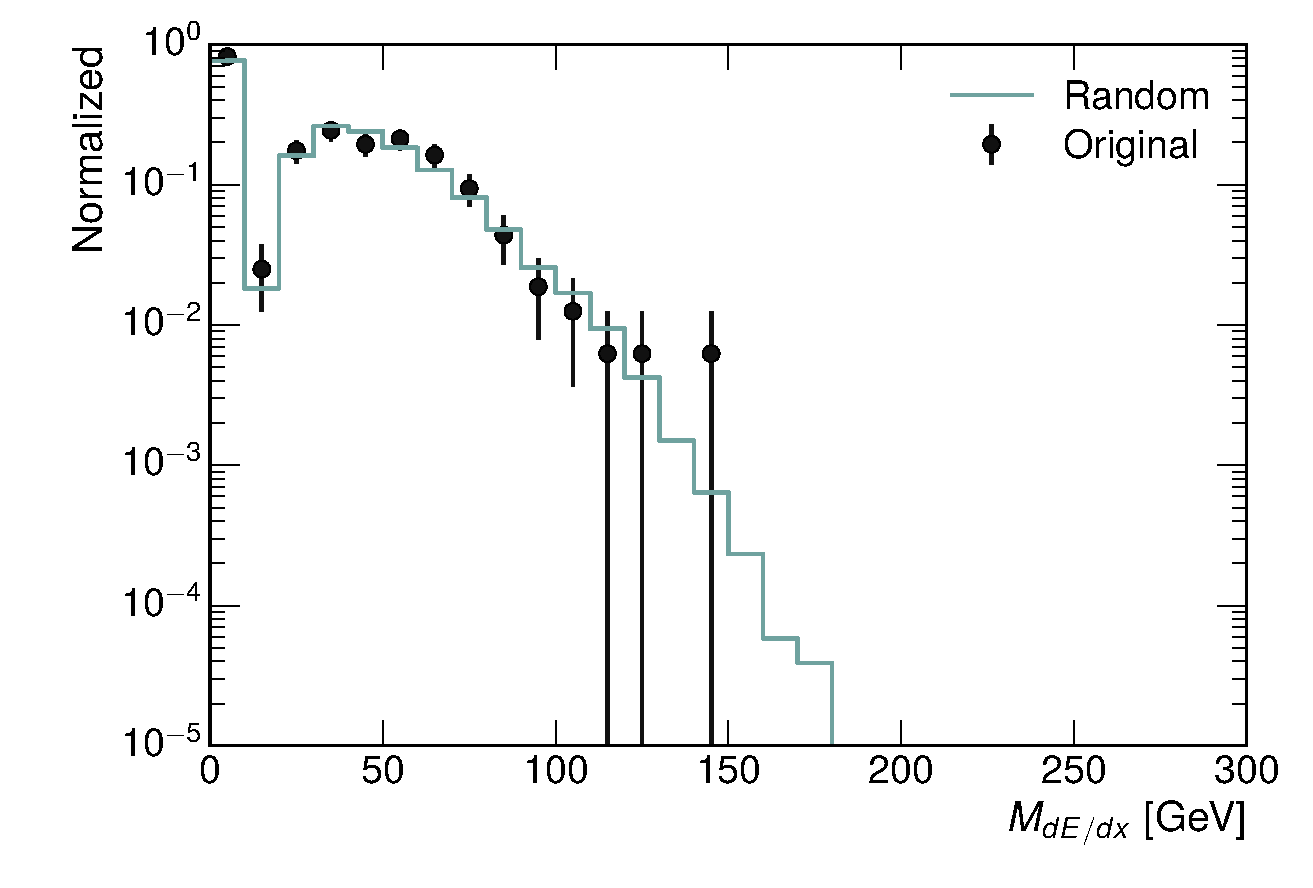
\includegraphics[width=\halffig]{figures/validation_mass_noion.pdf}
}
\subfloat[]{
  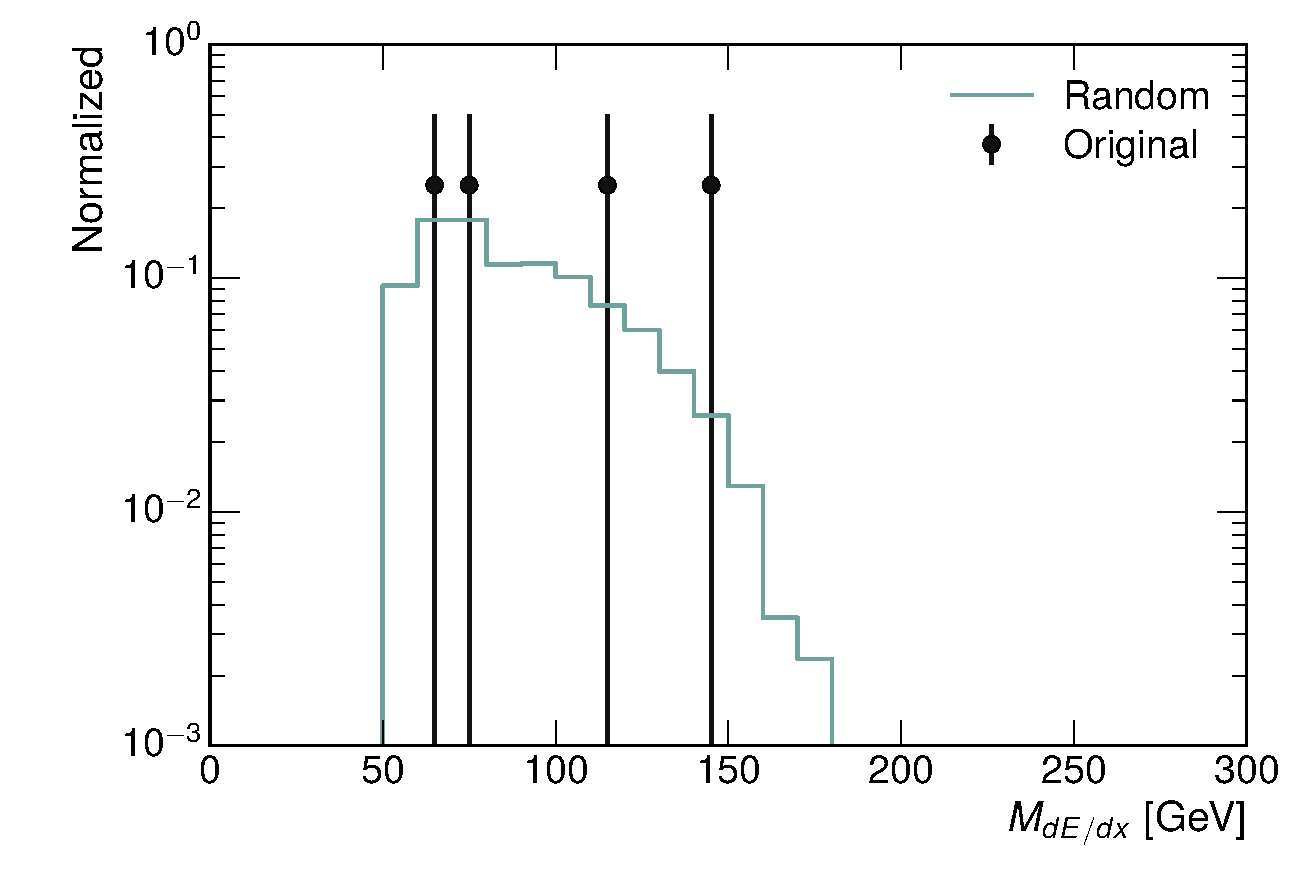
\includegraphics[width=\halffig]{figures/validation_mass.pdf}
}\\
\caption{The distribution of \mdedx (a) before and (b) after the ionization requirement for tracks in the validation region and for the randomly generated background estimate.}
\label{fig:validation_mass}
\end{figure}
% ----------------------------------------


\section{Expected Background}

Using the full technique in the primary regions described in Section~\ref{sec:background_method} provides a final background estimate for the signal region of this search.
It predicts a total background of 11.1 $\pm$ 1.7 events in the \ac{LL} region and 17.2 $\pm$ 2.6 events in the \ac{VLL} region.
Table~\ref{tab:background_yields} shows the number of events predicted in mass windows for the grid of mass points, for each of the \ac{LL} and \ac{VLL} signal regions.
Only one to two events are expected in each mass window, as the background distribution falls with increasing mass.

\begin{table}
\centering
\begin{tabular}{crr}
  \hline
  Mass & Expected Background, \acs*{LL} & Expected Background, \acs*{VLL} \\
  \hline
  1000 & $1.328 \pm 0.063 $ & $1.803 \pm 0.081 $ \\
  1100 & $1.255 \pm 0.060 $ & $1.409 \pm 0.069 $ \\
  1200 & $1.193 \pm 0.058 $ & $1.310 \pm 0.066 $ \\
  1300 & $0.997 \pm 0.051 $ & $1.431 \pm 0.069 $ \\
  1400 & $1.131 \pm 0.056 $ & $1.273 \pm 0.065 $ \\
  1500 & $1.111 \pm 0.055 $ & $1.115 \pm 0.059 $ \\
  1600 & $1.193 \pm 0.058 $ & $1.041 \pm 0.057 $ \\
  1800 & $1.138 \pm 0.056 $ & $0.918 \pm 0.053 $ \\
  \hline
\end{tabular}
\caption{The expected number of background events within each of the mass windows for the \acs*{LL} and \acs*{VLL} signal regions.}
\label{tab:background_yields}
\end{table}

